% Template for ICASSP-2013 paper; to be used with:
%          spconf.sty  - ICASSP/ICIP LaTeX style file, and
%          IEEEbib.bst - IEEE bibliography style file.
% --------------------------------------------------------------------------
\documentclass{article}
\usepackage{spconf,amsmath,graphicx}
\usepackage{subfig}
% Example definitions.
% --------------------
\def\x{{\mathbf x}}
\def\L{{\cal L}}

% Title.
% ------
\title{Prostate Cancer Detection in H\&E Stained Tissue Images}
%
% Single address.
% ---------------
\name{Ayush Jain, Chinmay Kulkarni, Aditya Rastogi}
\address{\{ajain42, ckulkarn, arastog2\}@illinois.edu}
%
% For example:
% ------------
%\address{School\\
%   Department\\
%   Address}
%
% Two addresses (uncomment and modify for two-address case).
% ----------------------------------------------------------
%\twoauthors
%  {A. Author-one, B. Author-two\sthanks{Thanks to XYZ agency for funding.}}
%   {School A-B\\
%   Department A-B\\
%   Address A-B}
%  {C. Author-three, D. Author-four\sthanks{The fourth author performed the work
%   while at ...}}
%   {School C-D\\
%   Department C-D\\
%   Address C-D}

\begin{document}
%\ninept
%
\maketitle
%
\begin{abstract}
More than 220,000 new cases of prostate cancer are observed in North America. About 1 in 7 men are likely to be diagnosed with prostate cancer. The increased fous on early and periodic testing demands a lot from the limited number of pathologists. Automated techniques that are (i) able to identify cancerous cases, or (ii) prune away a majority of non-cancerous cases would help focus pathologists' attention on challenging cases. This work attempts to detect prostate cancer using H\&E stained prostate tissue images. The extraction of meaningful features leads to an accuracy of 82\% -- an improvement of 30\% over baseline.
\end{abstract}
%
\begin{keywords}
Prostate cancer, biopsy, machine learning, image processing
\end{keywords}
%


\section{Introduction}
\label{sec:introduction}

\subsection{Background}
Prostrate cancer is the second most common cancer
among men. Several screening methodologies exist for diagnosis of prostate cancer however it is most commonly diagnosed by histopathology interpretation of Hematoxylin and Eosin (H \& E)-stained tissue sections by pathologist under a microscope. Diagnosis of prostate cancer is carried out by examining the glandular architecture of the tissue sections. The diagnosis is done in the form of the Gleason grading system \cite{gleason1966classification} under which pathologists identify the malignancy of cancer areas in tissue images on a scale of 1 to 5.Gland distributions vary with the disease grade, and the morphological features of the glands vary with the stage of cancer. However, this is prone to subjectivity and has limited intra- and inter-pathologist reproducibility, due to its heavy reliance on human interpretation. Even if only a single grade is desired, recent work has discovered that there is only a 60-70 \% agreement between pathologists on this grade.


Existing techniques to perform automated analysis of H \& E stained tissue have not had much accuracy expect in stylized toy cases. And because of the inter-disciplinary nature of the task, the problem has not attracted much attention. Most of the research has focused on distinguishing between Gleason grades (often between only two Gleason grades).In our work we focus on distinguishing cancerous tissue from non-cancerous tissue rather than distinguishing between Gleason grades for the tissue.

\subsection{Prostate Tissue Structure}
Normal Prostate tissue shown in Figure \ref{fig:tissue_structure1} is composed of gland units contained inside a fibromuscular region called stroma which holds the gland units together. Each gland unit is composed of rows of epithelial cells located around a duct, named the lumen. 

Figure \ref{fig:tissue_types} shows non-cancerous and cancerous Prostate tissue. When cancer occurs the following changes take place in the tissue depending upon the level of malignancy:
\begin{enumerate}
\item[1.] Epithelial cells replicate in an uncontrolled way, disrupting the regular arrangement of gland units.
\item[2.] The glands in the cancerous region become small, regular, and more tightly packed as
cancer progresses from benign to highly malignant. While benign,healthy tissue has large and irregular lumen regions, higher grade cancers have small, narrow lumen regions.
\end{enumerate}


\begin{figure}[!htb]
\centering
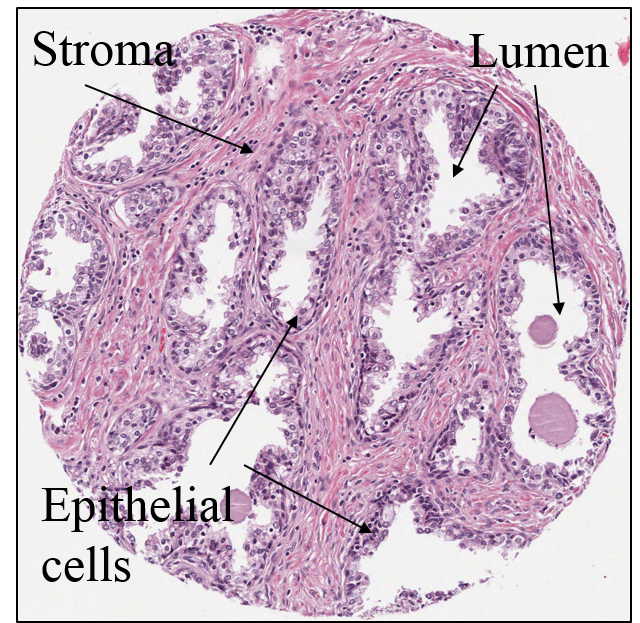
\includegraphics[scale=0.3]{figs/tissue_structure1.png}
\caption{Prostate Tissue Structure}\label{fig:tissue_structure1}
\centering
\end{figure}


\begin{figure}[!htb]
\centering
\captionsetup{justification=centering}
\begin{subfigure}{.5\textwidth}
	\centering
	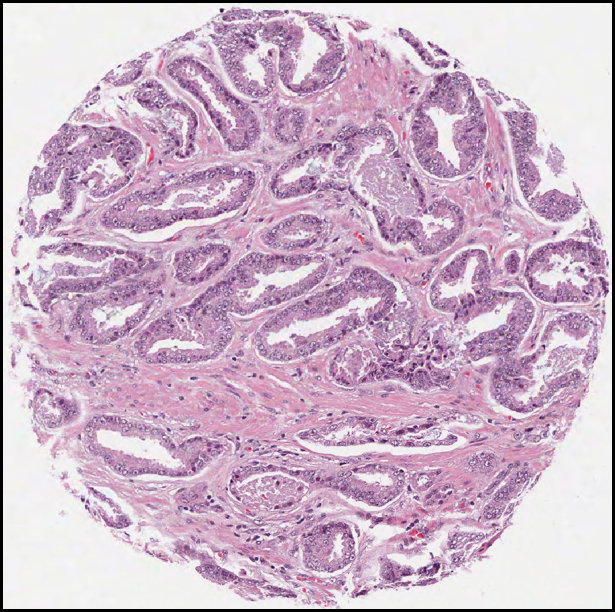
\includegraphics[scale=0.3]{figs/tissue_structure2.png}
	\caption{Benign Tissue}\label{fig:tissue_structure2}
	\centering
\end{subfigure}
\begin{subfigure}{.5\textwidth}
	\centering
	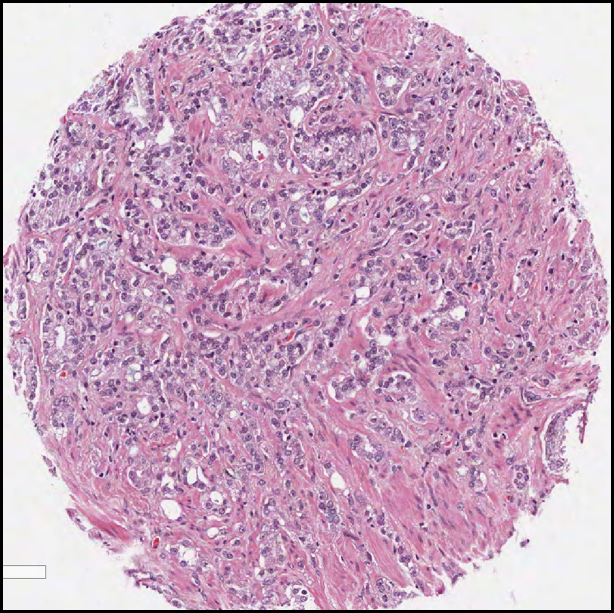
\includegraphics[scale=0.3]{figs/tissue_structure3.png}
	\caption{Malignant Tissue}\label{fig:tissue_structure2}
	\centering
\end{subfigure}
\caption{Structural changes in Prostate tissue when cancer occurs}
\label{fig:tissue_types}
\centering
\end{figure}

These changes, along with different color values identifying different regions of interest ( lumen regions are white, stroma is pink and epithelial cells are usually a dark shade of purple ) can be used to build a classification system for separating non-cancerous and cancerous images.

\section{Related Work}
There have been many different approaches tried for cancer detection in tissue stained images. \cite{automatic} segment parts of each image according to whether they are detected to be cancerous or not. In this paper, the authors make use of (Haralick features) in order to extract texture-based features. They use SVM-RFE for recursive feature selection which they apply to the entire image and evaluate their results using 10-fold cross-validation. The approach does not extract any features from the image or make use of any information about the structure of various components of the images. 
\cite{naik2007gland} make use of a more comprehensive approach. They segment parts of the image into detected gland components and subsequently extract morphological features from these components. To reduce the dimensionality of their data, they employ graph embedding and manifold learning. The features extracted for each image are very generic and do not capture much information specific to the differences in shape and size of various components of the image.
\cite{tabesh2007multifeature} make use of both morphological features as well as histogram-based features. They pre-process the images so that background colors are removed and so that the staining is made uniform. The striking fact about this paper is that they do not make use of any morphological features present in the various components of the image. In spite of using histogram-based features for their classification, the authors remove white pixels corresponding to lumen which is not intuitive. 
\cite{alexandratou2010evaluation} make use of Haralick features for extracting 13 texture characteristics using the Grey Level Co-occurence Matrix for images. They experiment with 16 different classifiers and run these classifiers over a very small data set or only about 40 images for cancer and non-cancer tissues. They obtain accuracy values of around 95\% for some of their classifiers, but the data set they use for classification is too small for this accuracy to make much sense.
The authors also count accuracy values for differentiating Gleason Score 3 and Gleason Score 4 images when they report their overall accuracy, when in fact this kind of distinction is a much easier task than differentiating cancerous images from non-cancerous images.
\cite{roula2002multispectral} make use of a novel approach wherein instead of analyzing RGB or grey scale images, they make use of the same feature vectors for a set of 16 spectral color bands. The authors apply a supervised classical Linear Discrimination method on the PCA result of the resultant combined feature vector (which is a linear combination of feature vectors for each color band) and show that the classification accuracy improves when using this spectral approach. The original feature vector contained texture-based features extracted using Haralick features. They observe better performance using the combined feature vector for 16 spectral bands over the original feature vector. The main drawback of this approach is that they are tweaking the data collection itself by observing each image as a combined feature vector of its 16 different spectral bands.

In most of the work done so far, not much effort has been put into capturing morphological features that are representative of different components of the image (lumen glands, epithelial cells and stroma). Most approaches discussed above make use of generic texture-based features without any specific processing or feature engineering for different image segments. Moreover, except for the last approach, all approaches make use of a limited number of images for testing their classifiers. In our work, we aim to focus the bulk of our effort on constructing effective and intuitive features for solving this problem. This leads to more robust features and our approach thus yields high accuracy values over data sets which are larger than those used in previous work.
\label{sec:rel_work}
\section{Patch-Based Approaches}
\label{sec:patch_based_approaches}
\section{Classification Using Image-Level Features}
The approaches using patch-based features failed to capture features that spanned multiple patches and which were representative of global characteristics of the images. 
In order to capture these characteristics, it was necessary to segment the images to separate out components that corresponded to epithelial cells and lumen glands. 
Once these components were extracted from each image, features specific to each component could then be constructed. Parts of the image corresponding to stroma were not very distinctive features and thus we did not extract stroma regions.

\subsection{Image Segmentation}

\subsubsection{Lumen Gland Segmentation}

In order to detect lumen glands from each image, a k-Nearest Neighbors classifier was trained using 1800 pixels manually labelled from different components of the image. This training set consisted of an equal number of pixels that belonged to either stroma, lumen glands and epithelial cells. For each pixel in the image, we found its nearest neighbors in the RGB color space. Based on the distance in the color space of each pixel's neighborhood from pixels corresponding to stroma and epithelial cells, we assigned a probability of belonging to stroma to each pixel. Pixels that had probabilities less than a threshold (< 0.2) were thus classified as being part of lumen glands and the resultant images were converted to binary images indicating whether a pixel belonged to a lumen gland or not. This approach also detected the edges of the image as lumen glands since they have similar color intensities as lumen objects. Thus, the largest connected components in the resultant lumen segmented images were discarded as these belonged to image edges. Finally, lumen glands were smoothed out through dilation using a disk structuring element.

\subsubsection{Epithelial Cell Segmentation}

Various approaches were tried in order to extract pixels corresponding to epithelial cells. Initially, all the images were contrast enhanced by clipping intensity values below a given threshold and increasing the pixel intensities of the resulting pixels. This helped to distinguish pixels corresponding to epithelial cells from the rest of the image since these pixels had predominantly higher pixel intensities. Once this pre-processing was done, we tried extracting epithelial cells using 3 different approaches.

\begin{enumerate}

\item \textbf{Local Minima Approach:}\\
We convolved the image with a Laplacian of Gaussian filter observed high responses for regions corresponding to epithelial cells due to their circular shape. Subsequently, local maxima points were detected in a small window size for these high response pixels and only the largest response values were retained. The resulting binary image thus clearly segmented pixels corresponding to epithelial cells. The problem with this approach was that it failed to capture the connected components corresponding to epithelial cells and only represented these cells as single pixel responses. Two more approaches were thus tried which avoided this problem.

\item \textbf{K-Means Approach:}\\
In order to capture epithelial cells of varying sizes, Laplacian of Gaussian filters of different sizes were used. 8 different LoG filters of $\sigma$ and $3 \sigma$ for basic scales of $\sigma = \{\sqrt{2}, 2, 2\sqrt{2}, 4\}$ were used from the Leung-Malik Filter Bank \cite{lmfb}. On convolving the pre-processed images with these 8 LoG filters, we observed better detection of circular regions. K-means was applied on these images to separate out different structural components. We observed the most distinctive separation of clusters for $K = 8$. This is intuitive since it was observed that images consisted of different pixel intensities for the following 8 regions in general:

\begin{enumerate}

\item Lumen regions.
\item Outer shell of the epithelial cells (generally darker than the entire cell itself).
\item Inner parts of the epithelial cells.
\item Darker regions in the stroma which are located close to epithelial cells.
\item Image corners which are completely white.
\item Cytoplasm present inside lumen objects.
\item Darker staining of lumen objects along their gland walls.
\item Lighter staining of stroma cells in contact with the peripheral of the image.

\end{enumerate}

In order to detect the cluster that corresponded most closely to epithelial cells, we chose clusters with the smallest variance in size of connected components and those which had the smallest size overall since both these features were intuitive of a cluster belonging to epithelial cells. The circularity of connected components within a cluster was also used in order to make this decision and for doing this, an elliptical structuring element was used and connected components were dilated with this element. We observed that the drawback for this approach was the accuracy in correctly detecting the cluster corresponding to epithelial cells.

\item \textbf{Hough Transform Approach:}\\
Finally, we also tried another approach to detecting epithelial cells which involved using the Hough Transform \cite{hough} for detecting circular objects in the pre-processed images. The radius range of circles to be detected was based on the minimum and maximum epithelial cell radii that we observed in our images. Once circle centers were detected, we convolved each binary image with a circular structuring element to represent the approximate shape of epithelial cells.

\end{enumerate} 


\subsection{Feature Extraction}
After having extracted the lumen and epithelial components for each image, we constructed features on these components. The final feature vector involved 10 features extracted from lumen glands and 2 features extracted from epithelial cells.

\subsubsection{Lumen-Based Features}
Lumen glands play a key role in distinguishing non-cancerous tissues from cancerous tissues. We have constructed 10 morphological features from the lumen glands that we detect from images.

\begin{enumerate}
\item \textbf{Lumen Area Ratio:} The percentage of pixels in the entire image that correspond to lumen glands as compared to the total number of pixels in the image. In non-cancerous tissues, lumen glands generally occupy a larger proportion of the image area than in cancerous tissues and this feature will help capture this property effectively.

\item \textbf{Number of Lumen Objects:} This feature captures the total number of connected components that correspond to lumen objects. Though the proportion of the image area that corresponds to lumen objects is higher in non-cancerous tissues, the number of such lumen objects is low as compared to images of cancerous tissues. In cancerous tissue images, lumen objects are broken up due to an explosive growth of epithelial cells and thus we would expect them to contain more number of lumen objects than images of non-cancerous tissues.

\item \textbf{Average and Variance in Lumen Size:} By providing a measure of how large the average lumen object is and how varied the sizes of lumen objects are, we can distinguish global-level features that capture the size of lumen objects in general. We would expect non-cancerous tissue images to have larger average size of lumen objects and also much larger variance in the size of lumen objects. In cancerous tissue images, lumen objects are generally of similar size and are smaller on an average.

\item \textbf{Average and Variance in Circularity of Lumen Objects:} The circularity of lumen objects capture how regularly shaped they are. Circularity is defined as:\\
\begin{align*}
C = \fract{P^2}{A}
\end{align*}
where $C$ is the circularity of a lumen object, $P$ is its perimeter and $A$ defines the area of the lumen object.
The circularity for an irregularly shaped object will be higher than that of a regularly shaped one.
The intuition behind keeping this feature is that non-cancerous tissues generally show more irregularly shaped lumen objects and thus, we expect that the average and variance in circularity of lumen objects for these images would be larger than the corresponding values for cancerous tissue images.

\item \textbf{Average and Variance in Eccentricity of Lumen Objects:} This feature would give higher values for images in which the lumen objects are more elliptical in shape. In images of cancerous tissues, since lumen objects are more circular in nature, we would expect this feature value to be low. For non-cancerous tissue images on the other hand, this feature value is expected to be high in general.

\item \textbf{Average and Variance in Distance from Centroid:} We calculate the average and variance in the distance of boundary pixels of lumen objects from the corresponding centroid of these lumen objects. This feature was included to capture the trend in radii values for all boundary pixels of lumen objects, rather than just the maximum and minimum radii (as have already been captured using eccentricity). Non-cancerous tissue images are expected to have higher values for this feature than cancerous tissue images.

\end{enumerate}

\subsubsection{Epithelial Cell-Based Features}
The extent of cancer progression in a prostate cancer tissue can be characterized by the proliferation of epithelial cells throughout the stroma. In cancerous tissues, epithelial cells generally penetrate lumen objects multiply uncontrollably thus leading to higher density of epithelial cells. Contrastingly in non-cancerous tissues, epithelial cells generally line the lumen objects without puncturing them. We aim to capture these properties and construct 2 features based on morphological properties of epithelial cells.

\begin{enumerate}
\item \textbf{Percentage of Epithelial Cells:} We calculate the percentage of image pixels that correspond to epithelial cells in the entire image. In cancerous tissue images, epithelial cells are more common as compared to non-cancerous tissue images and thus this feature can effectively capture this property.

\item \textbf{Percentage of Epithelial Cells Along Lumen Boundaries:} By calculating the percentage of the total epithelial cells that are along the lumen boundaries as compared to epithelial cells throughout the image in general, we will be able to distinguish images in which the density of epithelial cells is high along the lumen boundaries. As explained previously, non-cancerous tissue images have a high density of epithelial cells along the lumen boundaries than cancerous tissue images. 

\end{enumerate}

We thus obtain a 12-dimensional feature vector for each image example. Besides the above morphological features, we also tried using histogram-based features to capture color variations between cancerous and non-cancerous images. The intuition behind this was that in cancerous images, the color histogram should shift towards blue to account for a larger number of epithelial cells as compared to non-cancerous tissues. This distinction was not clearly observed in our images though, the reasons for which were twofold. Namely, the color staining was not uniform for epithelial cells (the outer regions for cells were generally darker than the core areas), and many non-cancerous tissue images with a large number of lumen objects also had many epithelial cells around the boundaries of these lumen objects. We thus discarded these features from our feature vector since they were unable to provide a good distinction between cancerous and non-cancerous tissue images.

\label{sec:image_based_approaches}
\section{Evaluation}
\label{sec:evaluation}
\section{Conclusions}
\label{sec:conclusions}



% References should be produced using the bibtex program from suitable
% BiBTeX files (here: strings, refs, manuals). The IEEEbib.bst bibliography
% style file from IEEE produces unsorted bibliography list.
% -------------------------------------------------------------------------

%\nocite{*}
\bibliographystyle{IEEEbib}
\bibliography{refs}

\end{document}
